\documentclass[aspectratio=169]{beamer}

\usepackage{graphicx}
\usepackage{amsmath,amssymb}
\usepackage{ragged2e}
\usepackage{tikz}
\usepackage{xcolor}
\usepackage{array}
\usepackage{booktabs}

\usetikzlibrary{arrows.meta,positioning,fit,calc}

\graphicspath{{figures/}{./figures/}}

\definecolor{maroon1}{rgb}{0.478, 0, 0.235}
\definecolor{lightgray}{rgb}{0.94,0.94,0.97}
\definecolor{lightgray2}{rgb}{0.5,0.5,0.5}
\definecolor{maccblue}{RGB}{28,74,117}
\definecolor{maccgreen}{RGB}{44,118,92}
\definecolor{maccred}{RGB}{156,58,52}

\usetheme{Copenhagen}
\usecolortheme[named=maroon1]{structure}

\setbeamerfont{caption}{size=\scriptsize}
\setbeamertemplate{navigation symbols}{}
\setbeamercolor{block body}{fg=black,bg=lightgray}
\setbeamercolor{block title}{fg=white,bg=maroon1}
\setbeamercolor{takeawaybox}{fg=black,bg=maroon1!8}

\newcommand{\refnote}[1]{{\bfseries\color{maroon1}\scriptsize (#1)}}
\newcommand{\takeawaybox}[1]{%
\vspace{0.03cm}
\begin{center}
\begin{beamercolorbox}[wd=0.94\textwidth,sep=3pt,center,rounded=true,shadow=false]{takeawaybox}
\scriptsize
\textbf{\textcolor{maroon1}{Takeaway:}} #1
\end{beamercolorbox}
\end{center}
}

\setbeamercolor{blue title}{fg=white,bg=maccblue}
\setbeamercolor{blue body}{fg=black,bg=maccblue!8}
\setbeamercolor{green title}{fg=white,bg=maccgreen}
\setbeamercolor{green body}{fg=black,bg=maccgreen!8}
\setbeamercolor{red title}{fg=white,bg=maccred}
\setbeamercolor{red body}{fg=black,bg=maccred!8}

\expandafter\def\expandafter\insertshorttitle\expandafter{%
\insertshorttitle\hfill%
\insertframenumber\,/\,\inserttotalframenumber}

\title[CSChE Lyapunov-RL]{%
\textbf{Lyapunov-Guided Reinforcement Learning\\
for Practical Polymer CSTR Control}}

\author[A. H. Hamedi]{%
A. H. Hamedi\\[-0.2ex]
{\scriptsize Supervisor: P. Mhaskar}}

\date[CSChE Draft]{%
{\scriptsize CSChE Conference Draft}\\[-0.1ex]
{\scriptsize Department of Chemical Engineering, McMaster University}}

\begin{document}

%============================= Slide 1 ============================
\begin{frame}
\setbeamertemplate{blocks}[rounded][shadow=false]
\setbeamercolor{block body}{fg=white,bg=maroon1}

\vspace{0.10cm}
\begin{center}

\includegraphics[width=.70\textwidth,height=0.22\linewidth,keepaspectratio]{logo.png}
\end{center}

\vspace{0.20cm}
\begin{block}{}
\begin{center}
\parbox{0.92\textwidth}{\centering
\Large \textbf{Lyapunov-Guided Reinforcement Learning\\
for Practical Polymer CSTR Control}}
\end{center}
\end{block}

\begin{center}
{\large \textbf{A. H. Hamedi}}\\[0.25ex]
{\scriptsize Supervisor: P. Mhaskar}\\[0.8ex]
{\scriptsize \color{maroon1} McMaster University}\\[0.45ex]
{\scriptsize \color{lightgray2} In collaboration with Linde plc.}
\end{center}
\end{frame}

%============================= Slide 2 ============================
\begin{frame}
\frametitle{\large \textbf{Technical objective: learn actions without losing certification}}
\small

\begin{columns}[T,onlytextwidth]
\begin{column}{0.50\textwidth}
\begin{block}{Closed-loop problem}
\[
x_{k+1}=f(x_k,u_k,p_k), \qquad y_k=h(x_k)
\]
\[
u_k=[Q_{c,k},Q_{m,k}]^\top,\qquad y_k=[\eta_k,T_k]^\top
\]
\[
u_{\min}\le u_k\le u_{\max}
\]
\end{block}

\begin{block}{Why chemical-process RL is difficult}
\begin{itemize}\justifying
  \setlength\itemsep{0.30ex}
  \item Slow dynamics make unsafe exploration expensive.
  \item Plant-model mismatch shifts the steady state.
\end{itemize}
\end{block}
\end{column}

\begin{column}{0.47\textwidth}
\begin{block}{Control objective}
Track a raw process setpoint while keeping the action certified:
\[
\min \sum_k \|y_k-y_{sp,k}\|_{Q_y}^2+\|\Delta u_k\|_{R_{\Delta u}}^2
\]
\[
V_{k+1}\le \rho V_k+\epsilon
\]
\end{block}

\begin{block}{Why MPC remains the baseline}
\begin{itemize}\justifying
  \setlength\itemsep{0.30ex}
  \item MPC optimizes predicted behavior under constraints.
  \item Lyapunov MPC adds a certificate, but depends on the selected target.
\end{itemize}
\refnote{Rawlings et al., 2017}
\end{block}
\end{column}
\end{columns}

\takeawaybox{The technical question is how to let TD3 propose useful moves while the Lyapunov layer certifies or replaces each move online.}
\end{frame}

%============================= Slide 3 ============================
\begin{frame}
\frametitle{\large \textbf{Polymer CSTR tracking is multivariable and scaled}}
\scriptsize

\begin{columns}[T,onlytextwidth]
\begin{column}{0.40\textwidth}
\begin{center}
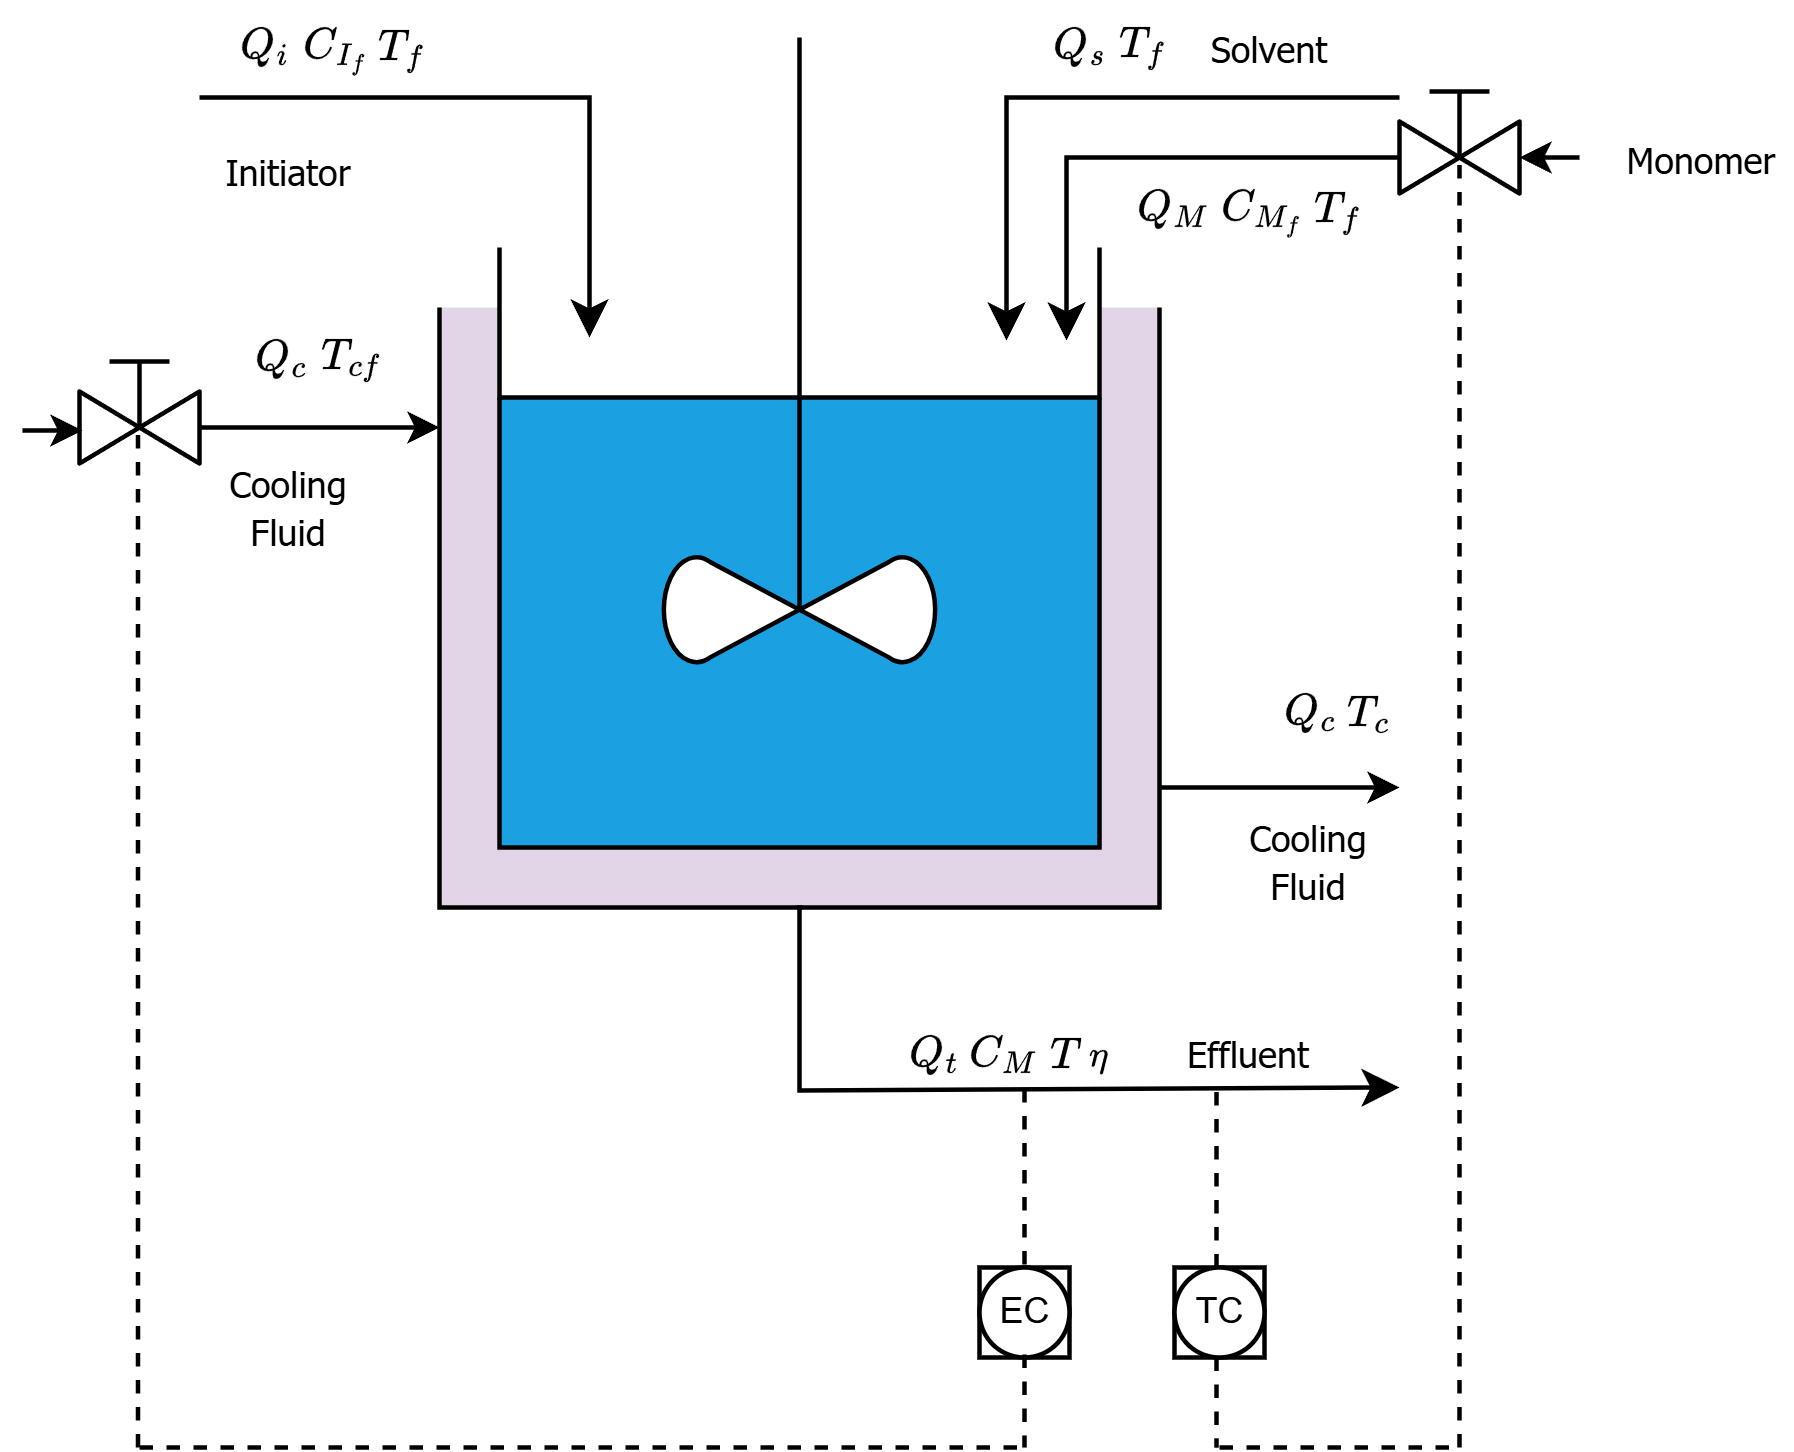
\includegraphics[width=0.92\textwidth]{CSTR.png}
\end{center}
\end{column}

\begin{column}{0.57\textwidth}
\begin{block}{Variables}
\begin{itemize}\justifying
  \setlength\itemsep{0.35ex}
  \item Manipulated input:
  \[
  u_k^{\rm phys}=[Q_{c,k}, Q_{m,k}]^\top
  \]
  \item Controlled output:
  \[
  y_k^{\rm phys}=[\eta_k, T_k]^\top
  \]
  \item Controller calculations use scaled deviations:
  \[
  \Delta y_k=S(y_k^{\rm phys})-S(y_{\rm ss}^{\rm phys})
  \]
\end{itemize}
\end{block}

\begin{block}{Latest analyzed disturbance run}
\begin{itemize}\justifying
  \setlength\itemsep{0.35ex}
  \item Two setpoint blocks per episode.
  \item Setpoint block length is 400, giving 800 steps per episode.
  \item Latest report analyzes 300 episodes and a final evaluation episode.
\end{itemize}
\end{block}
\end{column}
\end{columns}

\takeawaybox{The plant is simulated in physical units, but MPC, Lyapunov checks, and TD3 actions are evaluated in scaled deviation coordinates.}
\end{frame}

%============================= Slide 4 ============================
\begin{frame}
\frametitle{\large \textbf{Offset-free control needs a moving steady target}}
\scriptsize

\begin{columns}[T,onlytextwidth]
\begin{column}{0.52\textwidth}
\begin{block}{Augmented observer}
Let $\hat z_k=[\hat x_k,\hat d_k]^\top$. The controller model uses:
\[
\hat z_{k+1}=A_{\rm aug}\hat z_k+B_{\rm aug}\Delta u_k
\]
\[
\hat y_k=C_{\rm aug}\hat z_k
\]
\[
\hat z_{k+1}\leftarrow \hat z_{k+1}+L(\Delta y_k-C_{\rm aug}\hat z_k)
\]
\end{block}

\begin{block}{Why the target matters}
\begin{itemize}\justifying
  \setlength\itemsep{0.35ex}
  \item The controller does not only choose a move.
  \item It also chooses a steady center for tracking and Lyapunov decrease.
  \item Poor target centering can make a stable controller track the wrong objective.
\end{itemize}
\end{block}
\end{column}

\begin{column}{0.45\textwidth}
\begin{center}
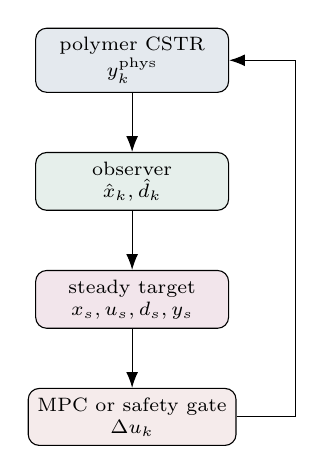
\begin{tikzpicture}[node distance=0.75cm, every node/.style={font=\scriptsize}]
\tikzstyle{box}=[draw, rounded corners, align=center, minimum width=2.45cm, minimum height=0.68cm, fill=lightgray]
\node[box, fill=maccblue!12] (plant) {polymer CSTR\\$y_k^{\rm phys}$};
\node[box, below=of plant, fill=maccgreen!12] (obs) {observer\\$\hat x_k,\hat d_k$};
\node[box, below=of obs, fill=maroon1!10] (target) {steady target\\$x_s,u_s,d_s,y_s$};
\node[box, below=of target, fill=maccred!10] (mpc) {MPC or safety gate\\$\Delta u_k$};
\draw[-{Latex[length=2mm]}] (plant) -- (obs);
\draw[-{Latex[length=2mm]}] (obs) -- (target);
\draw[-{Latex[length=2mm]}] (target) -- (mpc);
\draw[-{Latex[length=2mm]}] (mpc.east) -- ++(0.75,0) |- (plant.east);
\end{tikzpicture}
\end{center}
\end{column}
\end{columns}

\takeawaybox{The target selector is part of the controller, not a harmless preprocessing step.}
\end{frame}

%============================= Slide 5 ============================
\begin{frame}
\frametitle{\large \textbf{Direct target selection freezes the disturbance estimate}}
\scriptsize

\begin{columns}[T,onlytextwidth]
\begin{column}{0.50\textwidth}
\begin{block}{Steady target package}
\[
(x_s,d_s,u_s,y_s)
\]
\[
x_s=A x_s+B u_s
\]
\[
y_s=Cx_s+d_s
\]
\[
d_s=\hat d_k
\]
\end{block}
\end{column}

\begin{column}{0.47\textwidth}
\begin{block}{Bounded target selection}
If the exact target violates input bounds, the bounded solver chooses an admissible steady target:
\[
\Delta u_{\min}\le u_s\le \Delta u_{\max}
\]
\[
\min \; \|y_s-y_{sp}\|^2
+ w_u\|u_s-u_{k-1}\|^2
+ w_x\|x_s-x_{s,k-1}\|^2
\]
\end{block}
\end{column}
\end{columns}

\begin{block}{Important limitation}
\justifying
A target can be feasible for the Lyapunov machinery and still be a poor center for raw setpoint tracking, especially when the frozen disturbance estimate and input bounds make the exact raw setpoint unreachable.
\end{block}

\takeawaybox{The unresolved issue is target quality, not only target feasibility.}
\end{frame}

%============================= Slide 6 ============================
\begin{frame}
\frametitle{\large \textbf{Direct Lyapunov MPC enforces first-step contraction}}
\scriptsize

\begin{columns}[T,onlytextwidth]
\begin{column}{0.53\textwidth}
\begin{block}{Tracking objective}
\[
\min_{\Delta u_{0:N-1}}
\sum_{i=0}^{N-1}
\left(
\|y_{k+i}-y_{sp,k+i}\|_{Q_y}^2
+\|\Delta u_{k+i}-\Delta u_{k+i-1}\|_{R_{\Delta u}}^2
\right)
\]
\[
\Delta u_{\min}\le \Delta u_{k+i}\le \Delta u_{\max}
\]
\end{block}
\end{column}

\begin{column}{0.44\textwidth}
\begin{block}{Lyapunov test}
The Lyapunov center is the selected target:
\[
e_k=\hat x_k-x_s
\]
\[
V_k=e_k^\top P e_k
\]
\[
V_{k+1}^{\rm first}\le \rho V_k+\epsilon
\]
Current report:
\[
\rho=0.99,\qquad \epsilon=10^{-2}
\]
\end{block}
\end{column}
\end{columns}

\begin{block}{Configuration note}
\justifying
Both $\epsilon=10^{-3}$ and $\epsilon=10^{-2}$ were tested. The latest report uses the more relaxed $\epsilon=10^{-2}$, which reduced gate activations but did not remove the target-selector limitation.
\end{block}

\takeawaybox{The certificate is only as useful as the Lyapunov center used to compute it.}
\end{frame}

%============================= Slide 7 ============================
\begin{frame}
\frametitle{\large \textbf{Safety-gated RL gives the actor authority, but not final authority}}
\scriptsize

\begin{center}
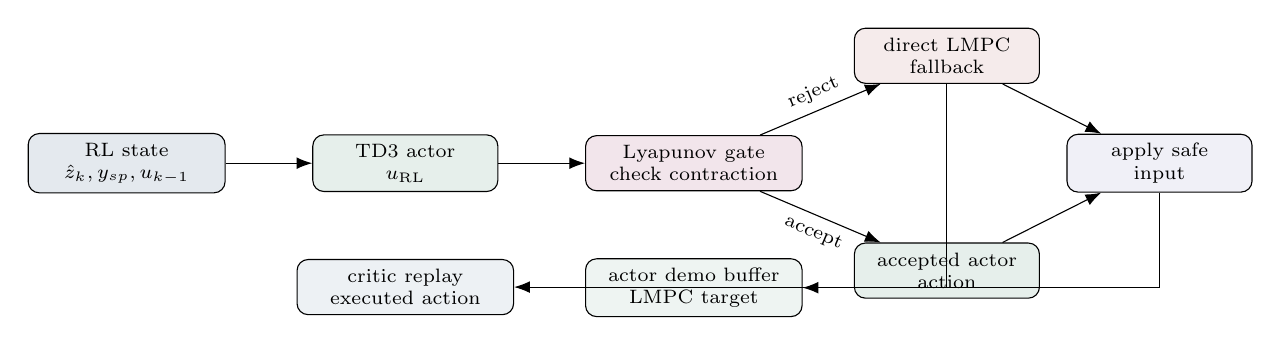
\begin{tikzpicture}[node distance=0.90cm and 1.10cm, every node/.style={font=\scriptsize}]
\tikzstyle{box}=[draw, rounded corners, align=center, minimum height=0.70cm, fill=lightgray]
\node[box, fill=maccblue!12, minimum width=2.5cm] (state) {RL state\\$\hat z_k,y_{sp},u_{k-1}$};
\node[box, fill=maccgreen!12, right=of state, minimum width=2.35cm] (actor) {TD3 actor\\$u_{\rm RL}$};
\node[box, fill=maroon1!10, right=of actor, minimum width=2.75cm] (gate) {Lyapunov gate\\check contraction};
\node[box, fill=maccred!10, above right=0.65cm and 0.65cm of gate, minimum width=2.35cm] (fallback) {direct LMPC\\fallback};
\node[box, fill=maccgreen!12, below right=0.65cm and 0.65cm of gate, minimum width=2.35cm] (accept) {accepted actor\\action};
\node[box, fill=lightgray, right=3.35cm of gate, minimum width=2.35cm] (plant) {apply safe\\input};
\node[box, fill=maccblue!8, below=0.85cm of actor, minimum width=2.75cm] (replay) {critic replay\\executed action};
\node[box, fill=maccgreen!8, below=0.85cm of gate, minimum width=2.75cm] (demo) {actor demo buffer\\LMPC target};

\draw[-{Latex[length=2mm]}] (state) -- (actor);
\draw[-{Latex[length=2mm]}] (actor) -- (gate);
\draw[-{Latex[length=2mm]}] (gate) -- node[above,sloped]{reject} (fallback);
\draw[-{Latex[length=2mm]}] (gate) -- node[below,sloped]{accept} (accept);
\draw[-{Latex[length=2mm]}] (fallback) -- (plant);
\draw[-{Latex[length=2mm]}] (accept) -- (plant);
\draw[-{Latex[length=2mm]}] (plant.south) |- (replay.east);
\draw[-{Latex[length=2mm]}] (fallback.south) |- (demo.east);
\end{tikzpicture}
\end{center}

\begin{block}{Agent-authority behavioral cloning}
\justifying
During BC, the actor still proposes the candidate action. Direct LMPC is computed separately as the imitation target for actor updates. The critic stores the executed safe action.
\end{block}

\takeawaybox{The learned controller is allowed to act from the beginning, but the Lyapunov gate protects the plant from rejected actions.}
\end{frame}

%============================= Slide 8 ============================
\begin{frame}
\frametitle{\large \textbf{Cold-start and pretrained RL test different learning priors}}
\scriptsize

\begin{columns}[T,onlytextwidth]
\begin{column}{0.48\textwidth}
\begin{beamercolorbox}[rounded=true,sep=4pt]{blue body}
\textbf{\textcolor{maccblue}{Cold-start RL}}
\begin{itemize}\justifying
  \setlength\itemsep{0.35ex}
  \item Actor begins without the pretrained policy prior.
  \item BC exploration is larger.
  \item Exploration decays from 0.2 to 0.01.
  \item TD3 policy smoothing noise is 0.1.
\end{itemize}
\end{beamercolorbox}
\end{column}

\begin{column}{0.48\textwidth}
\begin{beamercolorbox}[rounded=true,sep=4pt]{green body}
\textbf{\textcolor{maccgreen}{Pretrained RL}}
\begin{itemize}\justifying
  \setlength\itemsep{0.35ex}
  \item Actor starts closer to an OF-MPC-like behavior.
  \item BC exploration is smaller.
  \item Exploration decays from 0.02 to 0.01.
  \item TD3 policy smoothing noise is 0.01.
\end{itemize}
\end{beamercolorbox}
\end{column}
\end{columns}

\vspace{0.15cm}
\begin{block}{Training phases}
\begin{center}
\begin{tabular}{lccc}
\toprule
Phase & Episodes & Control role & Learning role \\
\midrule
Agent-authority BC & 1--20 & actor through gate & imitate LMPC target \\
Soft handoff & 21--25 & blended candidate through gate & transition to RL \\
Online TD3 & 26--299 & actor through gate & full TD3 updates \\
Final evaluation & 300 & actor through gate & no exploration \\
\bottomrule
\end{tabular}
\end{center}
\end{block}

\takeawaybox{Pretraining improves the early trajectory, while cold-start can eventually learn a more gate-compatible action style.}
\end{frame}

%============================= Slide 9 ============================
\begin{frame}
\frametitle{\large \textbf{Main result I: authority depends strongly on the learning phase}}
\scriptsize

\begin{columns}[T,onlytextwidth]
\begin{column}{0.60\textwidth}
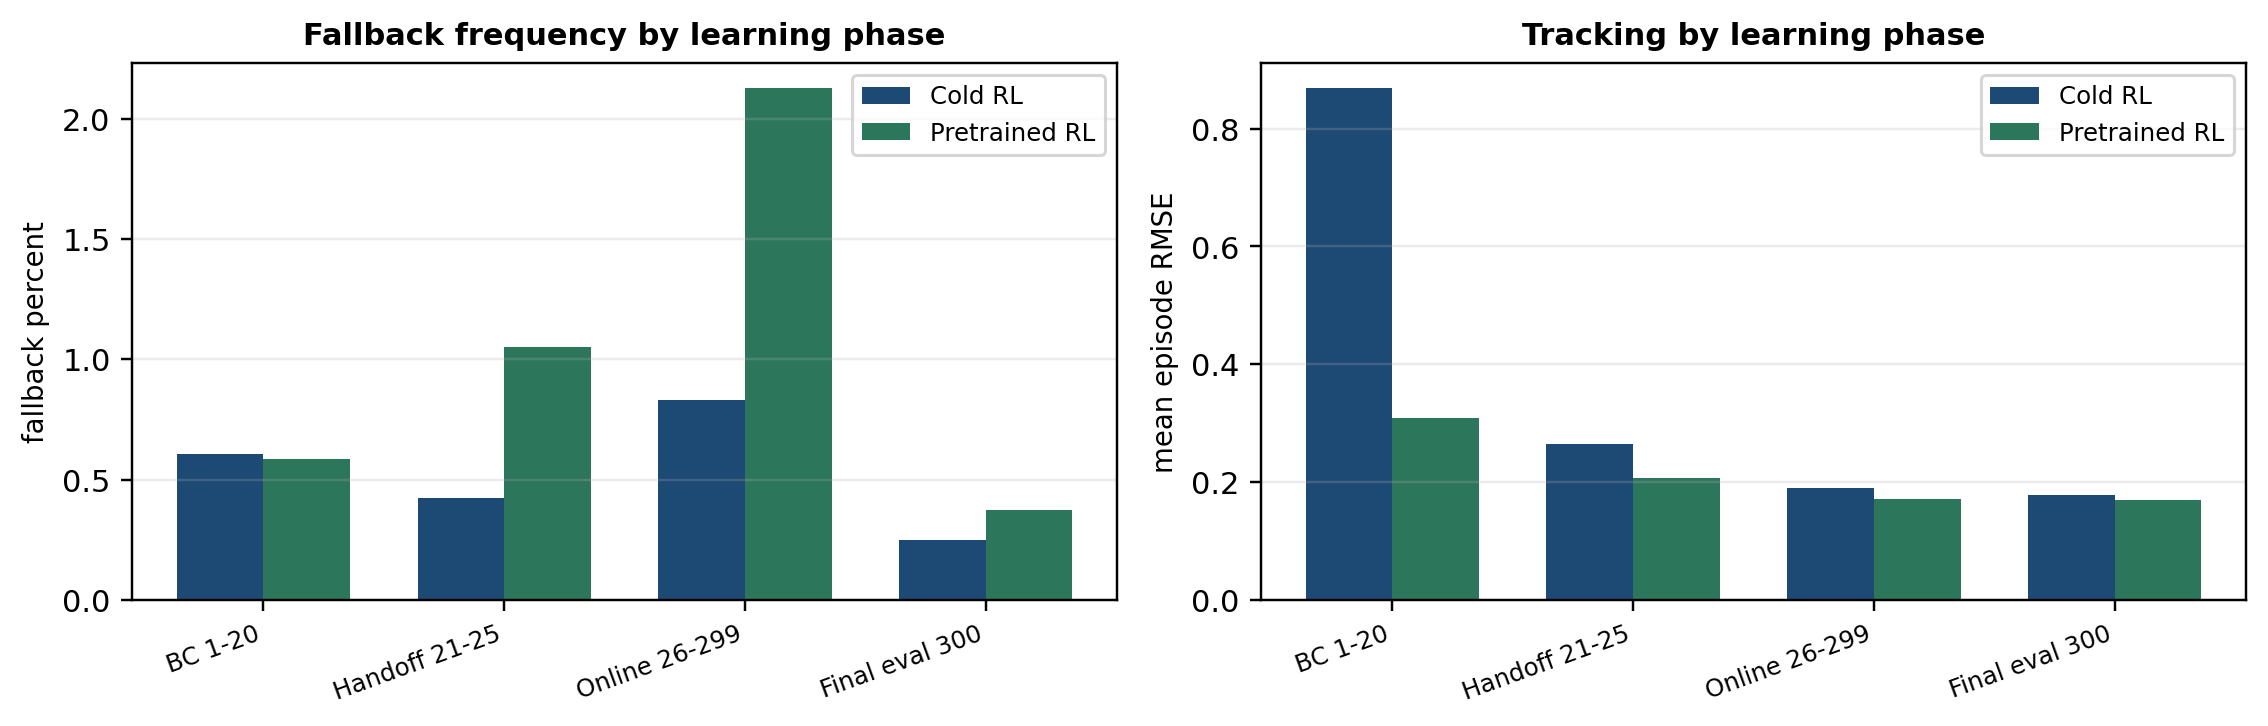
\includegraphics[width=\textwidth]{csche_phase_authority_summary.png}
\end{column}
\begin{column}{0.38\textwidth}
\begin{block}{Latest 300-episode report}
\begin{center}
\begin{tabular}{lcc}
\toprule
Case & Accepted & Fallback \\
\midrule
Cold RL & 99.11\% & 0.81\% \\
Pretrained RL & 97.92\% & 2.00\% \\
\bottomrule
\end{tabular}
\end{center}
\end{block}
\begin{block}{Technical reading}
\begin{itemize}\justifying
  \setlength\itemsep{0.35ex}
  \item BC is the fragile phase for cold-start RL.
  \item The final evaluation has low fallback for both agents.
  \item Pretrained RL tracks better, but uses the safety layer more over the full run.
\end{itemize}
\end{block}
\end{column}
\end{columns}

\takeawaybox{Cold-start has the stronger full-run authority signal, but pretraining gives the better tracking trajectory.}
\end{frame}

%============================= Slide 10 ============================
\begin{frame}
\frametitle{\large \textbf{Main result II: pretrained RL tracks better over the full horizon}}
\scriptsize

\begin{center}
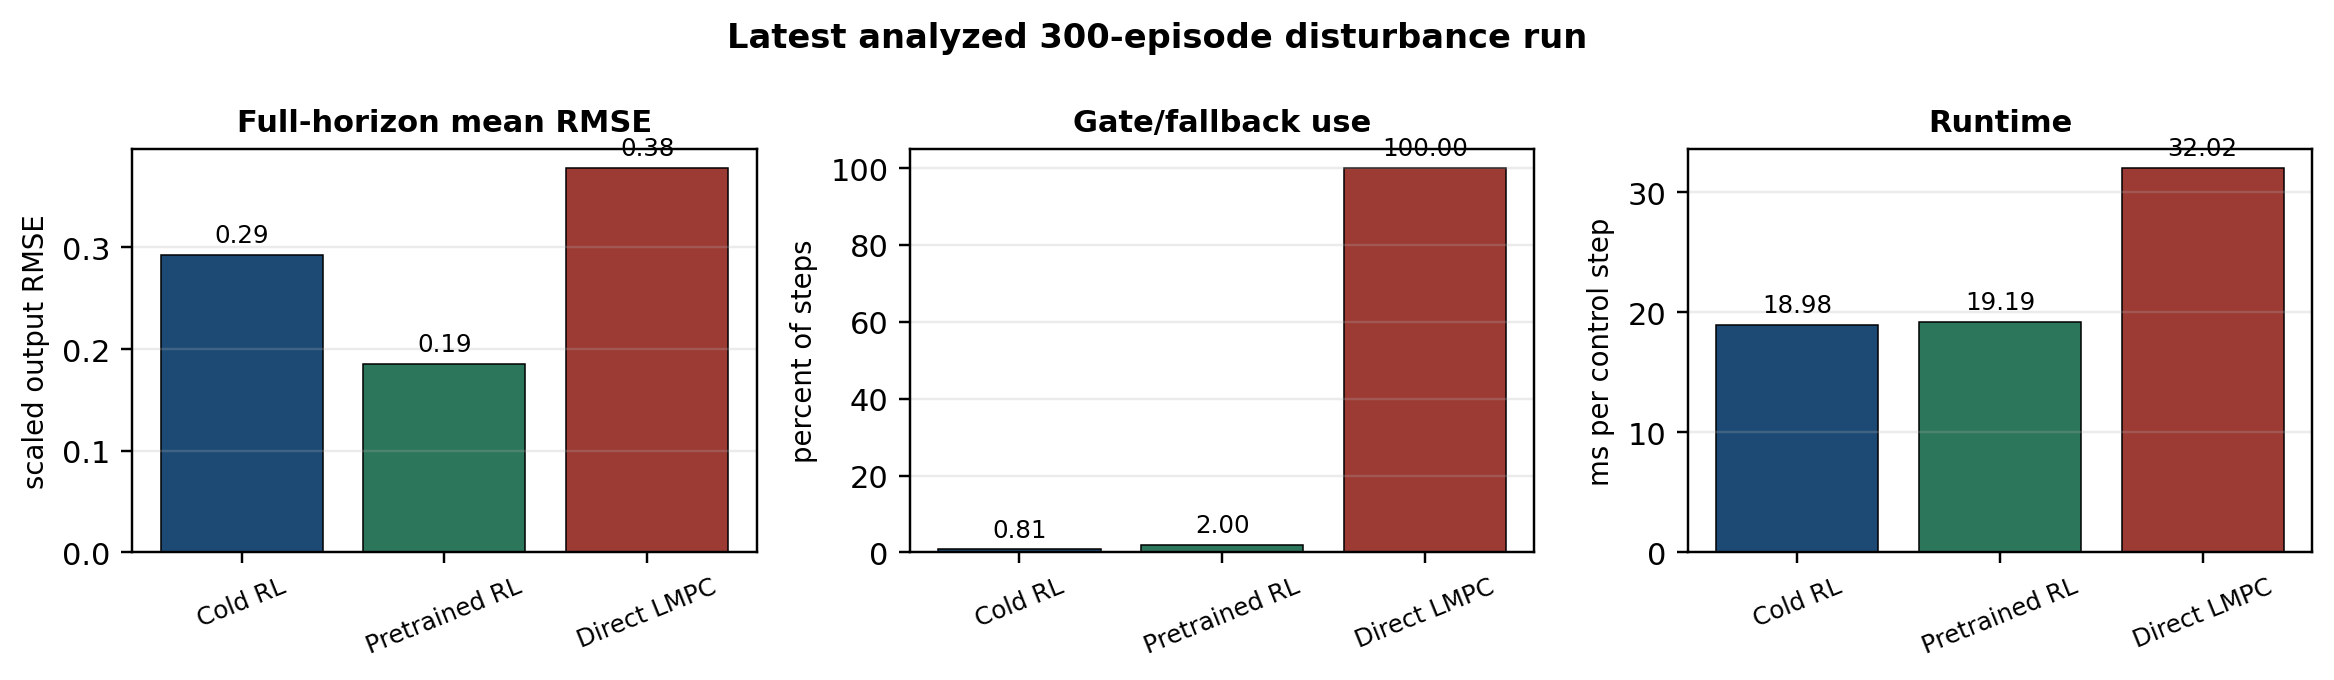
\includegraphics[width=0.93\textwidth]{csche_key_result_summary.png}
\end{center}

\vspace{-0.15cm}
\begin{block}{Numerical reading}
\begin{itemize}\justifying
  \setlength\itemsep{0.35ex}
  \item Mean RMSE: pretrained RL 0.185, cold RL 0.292, direct LMPC 0.378.
  \item Runtime: safety-gated RL is about 1.7 times faster per step than direct LMPC.
  \item Direct MPC-only is faster, but it is a diagnostic baseline without RL gating.
\end{itemize}
\end{block}

\takeawaybox{Pretraining gives better full-horizon performance, but the MPC-only diagnostic still shows that raw tracking can be better than the safety-gated policies.}
\end{frame}

%============================= Slide 11 ============================
\begin{frame}
\frametitle{\large \textbf{Final-tail behavior tells a different story than full-horizon RMSE}}
\scriptsize

\begin{center}
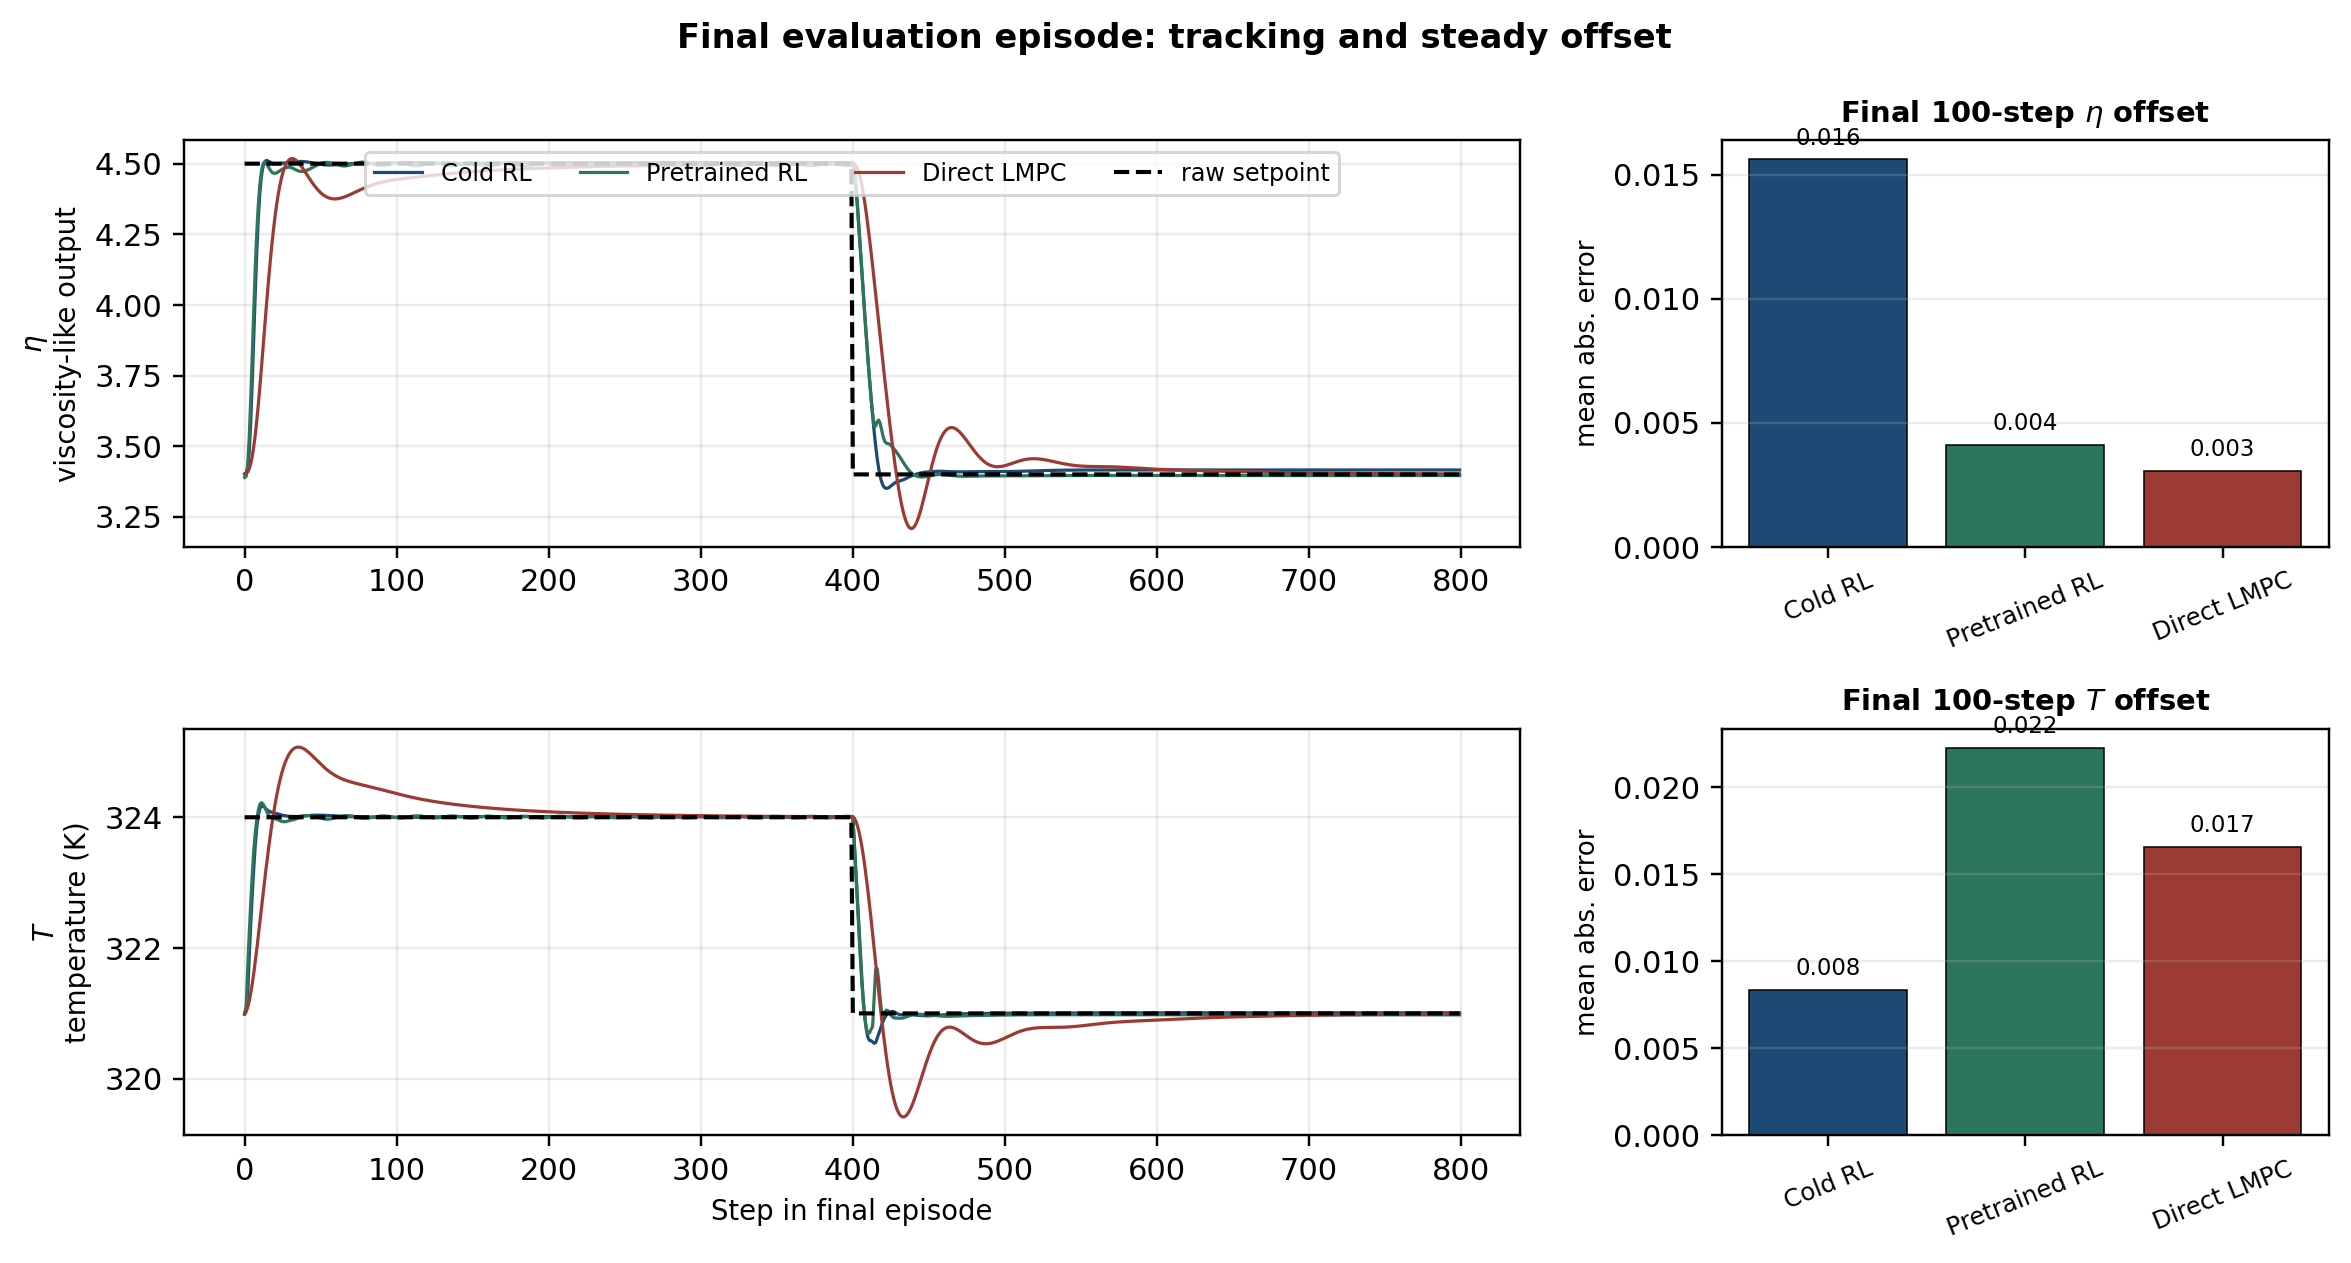
\includegraphics[height=0.66\textheight,keepaspectratio]{csche_final_episode_tracking_summary.png}
\end{center}

\takeawaybox{Direct LMPC can settle well in the final tail, while its full-horizon RMSE remains poor because the transient target path is slow or modified.}
\end{frame}

%============================= Slide 12 ============================
\begin{frame}
\frametitle{\large \textbf{The target selector is the current scientific bottleneck}}
\scriptsize

\begin{center}
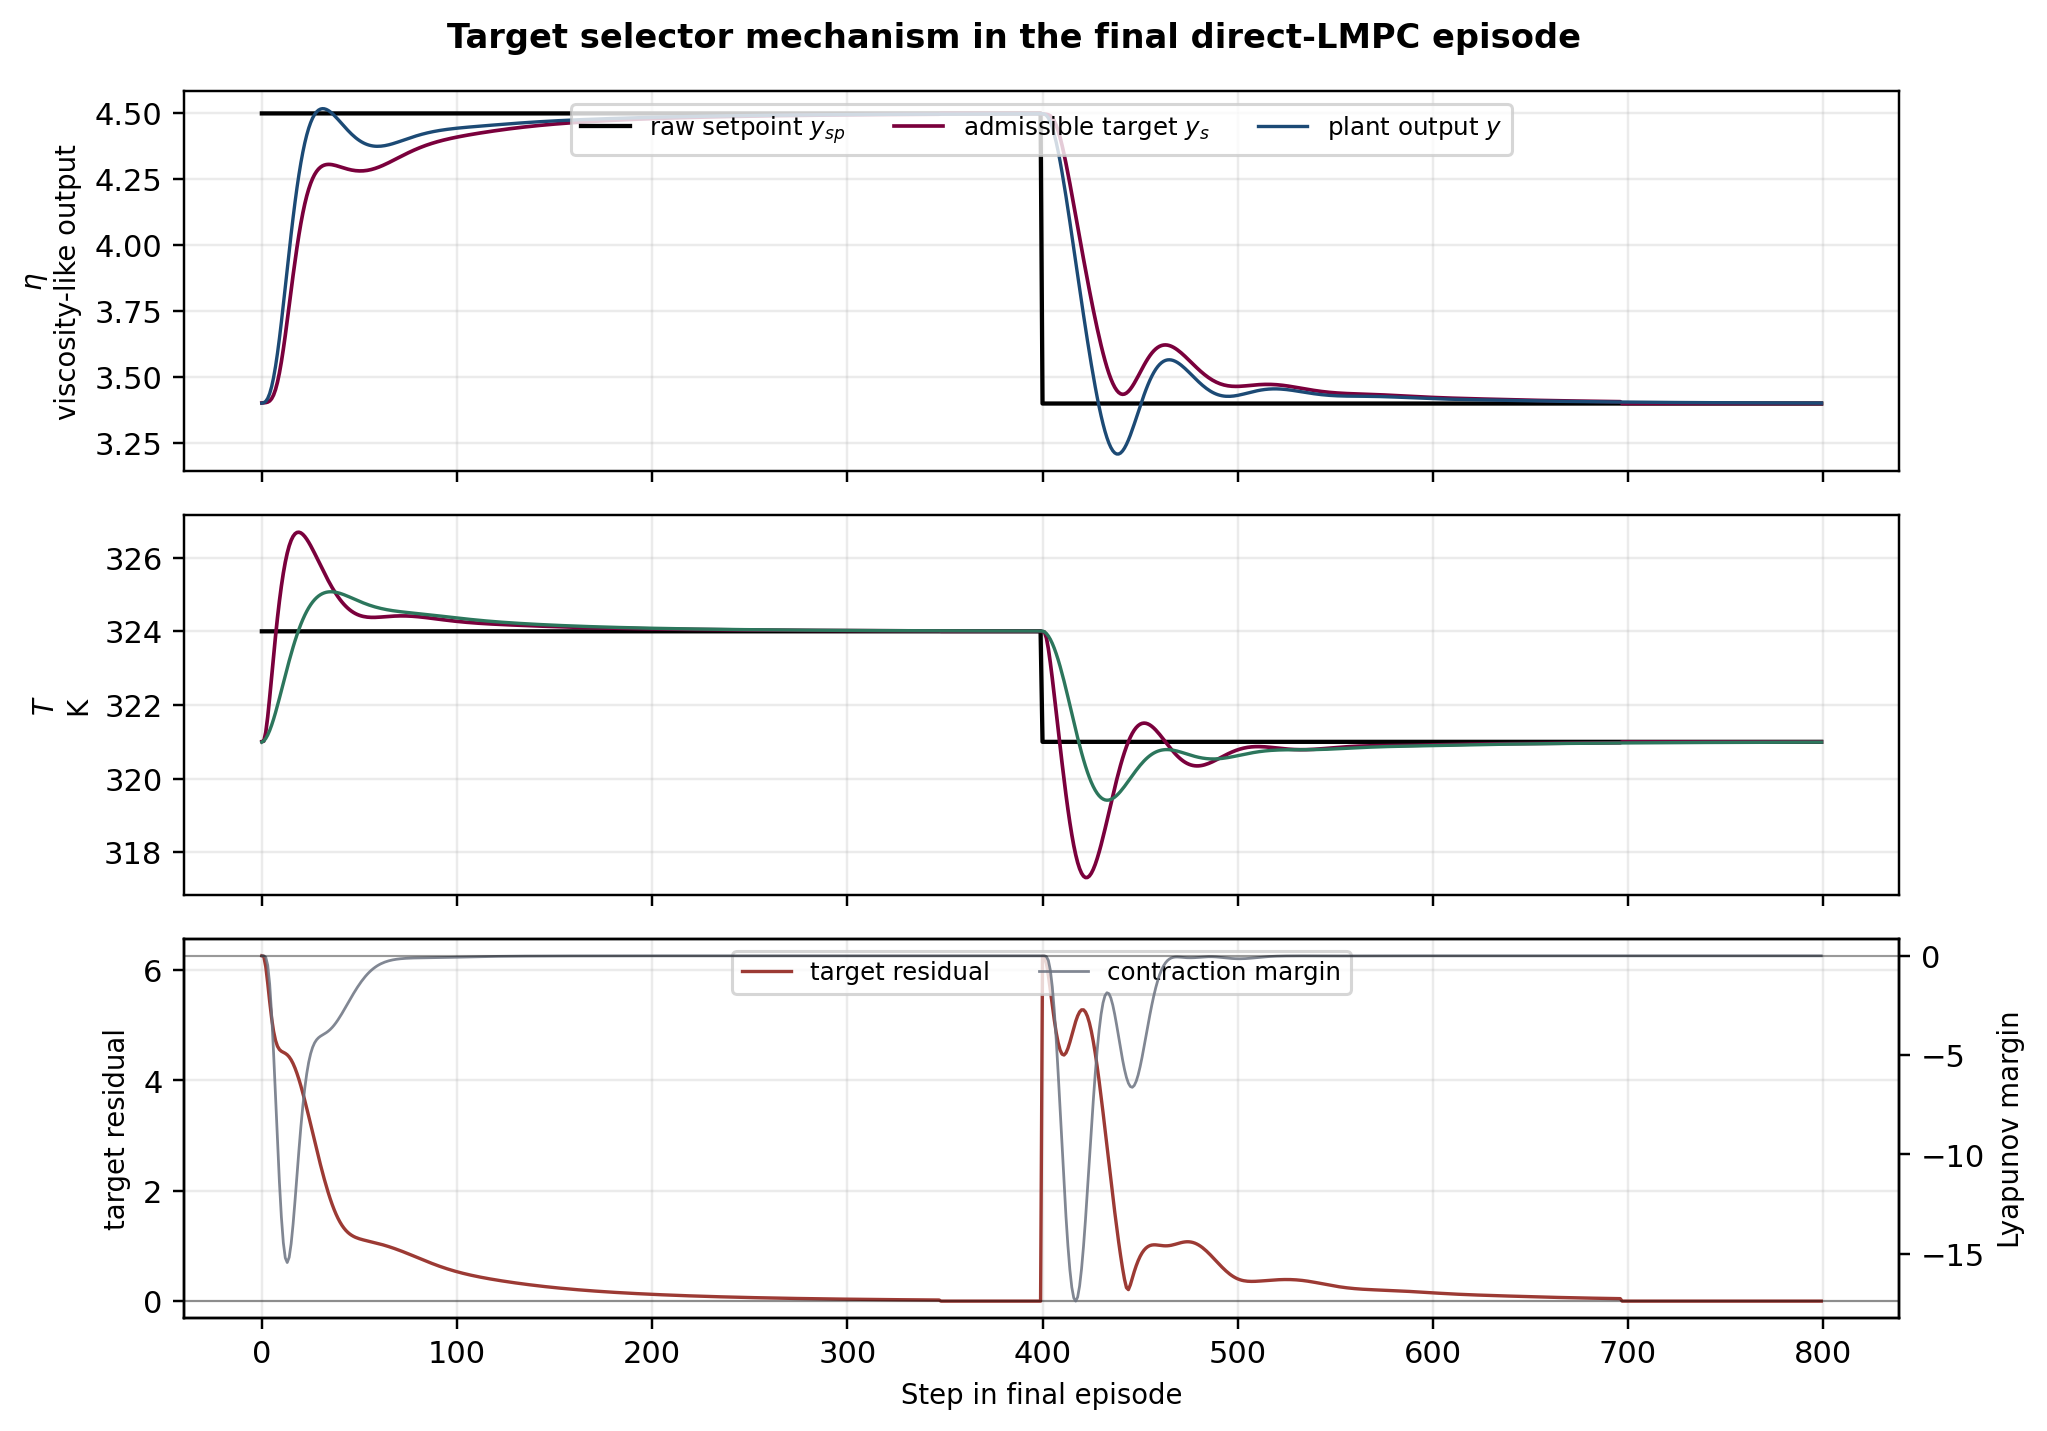
\includegraphics[height=0.66\textheight,keepaspectratio]{csche_target_selector_mechanism.png}
\end{center}

\takeawaybox{The bounded target can support contraction while drifting from the raw process objective. The key problem is choosing a Lyapunov target that is both admissible and aligned with $y_{sp}$.}
\end{frame}

%============================= Slide 13 ============================
\begin{frame}
\frametitle{\large \textbf{Scientific interpretation: what is working and what is not}}
\scriptsize

\begin{columns}[T,onlytextwidth]
\begin{column}{0.48\textwidth}
\begin{beamercolorbox}[rounded=true,sep=4pt]{green body}
\textbf{\textcolor{maccgreen}{Working}}
\begin{itemize}\justifying
  \setlength\itemsep{0.35ex}
  \item The actor can propose actions while the gate keeps final authority.
  \item Pretraining improves full-horizon reward and tracking.
  \item Timing instrumentation supports the practical speed benefit of RL plus gate over direct LMPC.
  \item MPC-only would-be activation now exposes hidden Lyapunov conflicts.
\end{itemize}
\end{beamercolorbox}
\end{column}

\begin{column}{0.48\textwidth}
\begin{beamercolorbox}[rounded=true,sep=4pt]{red body}
\textbf{\textcolor{maccred}{Unresolved}}
\begin{itemize}\justifying
  \setlength\itemsep{0.35ex}
  \item Admissible targets can be poor raw-setpoint centers.
  \item Reward and safety authority do not fully agree.
  \item Fallback penalties were increased, but this alone did not close the MPC-only gap.
  \item Relaxing $\epsilon$ helps activation rates, but does not solve target quality.
\end{itemize}
\end{beamercolorbox}
\end{column}
\end{columns}

\takeawaybox{The next step should be a target-selector experiment, not another broad reward-tuning sweep.}
\end{frame}

%============================= Slide 14 ============================
\begin{frame}
\frametitle{\large \textbf{Next experiment: ablate target quality directly}}
\scriptsize

\begin{block}{Small ablation plan}
\begin{enumerate}\justifying
  \setlength\itemsep{0.35ex}
  \item Baseline: current bounded direct target with $u_{k-1}$ and $x_{s,k-1}$ regularization.
  \item Hard target-quality guard: reject or hold when $\|y_s-y_{sp}\|_\infty$ exceeds a threshold.
  \item Two-layer selector: first choose the closest trackable raw target, then choose the least-moving Lyapunov center.
  \item Disturbance-regularized selector: allow small $d_s-\hat d_k$ only when it improves raw target alignment.
\end{enumerate}
\end{block}

\begin{block}{Metrics to compare}
\begin{center}
\begin{tabular}{lll}
\toprule
Tracking & Target quality & Safety and cost \\
\midrule
raw RMSE & $y_s-y_{sp}$ mismatch & fallback rate \\
final-tail offset & target residual & contraction margin \\
setpoint-block RMSE & target movement & wall-clock ms per step \\
\bottomrule
\end{tabular}
\end{center}
\end{block}

\takeawaybox{A successful target selector must improve raw setpoint tracking without hiding instability behind fallback or a softened contraction test.}
\end{frame}

%============================= Slide 15 ============================
\begin{frame}
\frametitle{\large \textbf{Closing message}}
\small

\begin{block}{One-sentence conclusion}
\justifying
The main challenge is no longer only learning a stabilizing action, but choosing a Lyapunov target that is both admissible and aligned with the raw process objective.
\end{block}

\vspace{0.12cm}
\begin{columns}[T,onlytextwidth]
\begin{column}{0.48\textwidth}
\begin{block}{What the framework provides}
\begin{itemize}\justifying
  \setlength\itemsep{0.35ex}
  \item MPC-compatible safety logic.
  \item Agent-authority RL with model-based fallback.
  \item Diagnostics for activation, target quality, and runtime.
\end{itemize}
\end{block}
\end{column}
\begin{column}{0.48\textwidth}
\begin{block}{What remains honest}
\begin{itemize}\justifying
  \setlength\itemsep{0.35ex}
  \item Current results are single-run simulation evidence.
  \item MPC-only still has better raw tracking in the analyzed run.
  \item Target selector design is still the central open problem.
\end{itemize}
\end{block}
\end{column}
\end{columns}

\vspace{0.1cm}
\begin{center}
{\large \textbf{Thank you}}
\end{center}
\end{frame}

\appendix

%============================= Backup 1 ============================
\begin{frame}
\frametitle{\large \textbf{Backup: reward used for the latest RL report}}
\scriptsize

\begin{block}{Reward structure}
The reward contains output error, move penalty, near-setpoint shaping, and fallback cost:
\[
r_k=r_{\rm track}+r_{\rm bonus}-J_{\rm move}-J_{\rm fb}
\]
\[
J_{\rm fb}=\gamma_{\rm fb}\sum_j R_{{\rm fb},j}g_j^2+c_{\rm fb}I_{\rm fb}
\]
\end{block}

\begin{columns}[T,onlytextwidth]
\begin{column}{0.50\textwidth}
\begin{block}{Latest active values}
\begin{itemize}
  \setlength\itemsep{0.25ex}
  \item $Q_y={\rm diag}(8,6)$
  \item $R_{\Delta u}={\rm diag}(1,1)$
  \item $\gamma_{\rm fallback}=3$
  \item $c_{\rm fb}=10$
  \item TD3 $\gamma=0.99$
\end{itemize}
\end{block}
\end{column}
\begin{column}{0.47\textwidth}
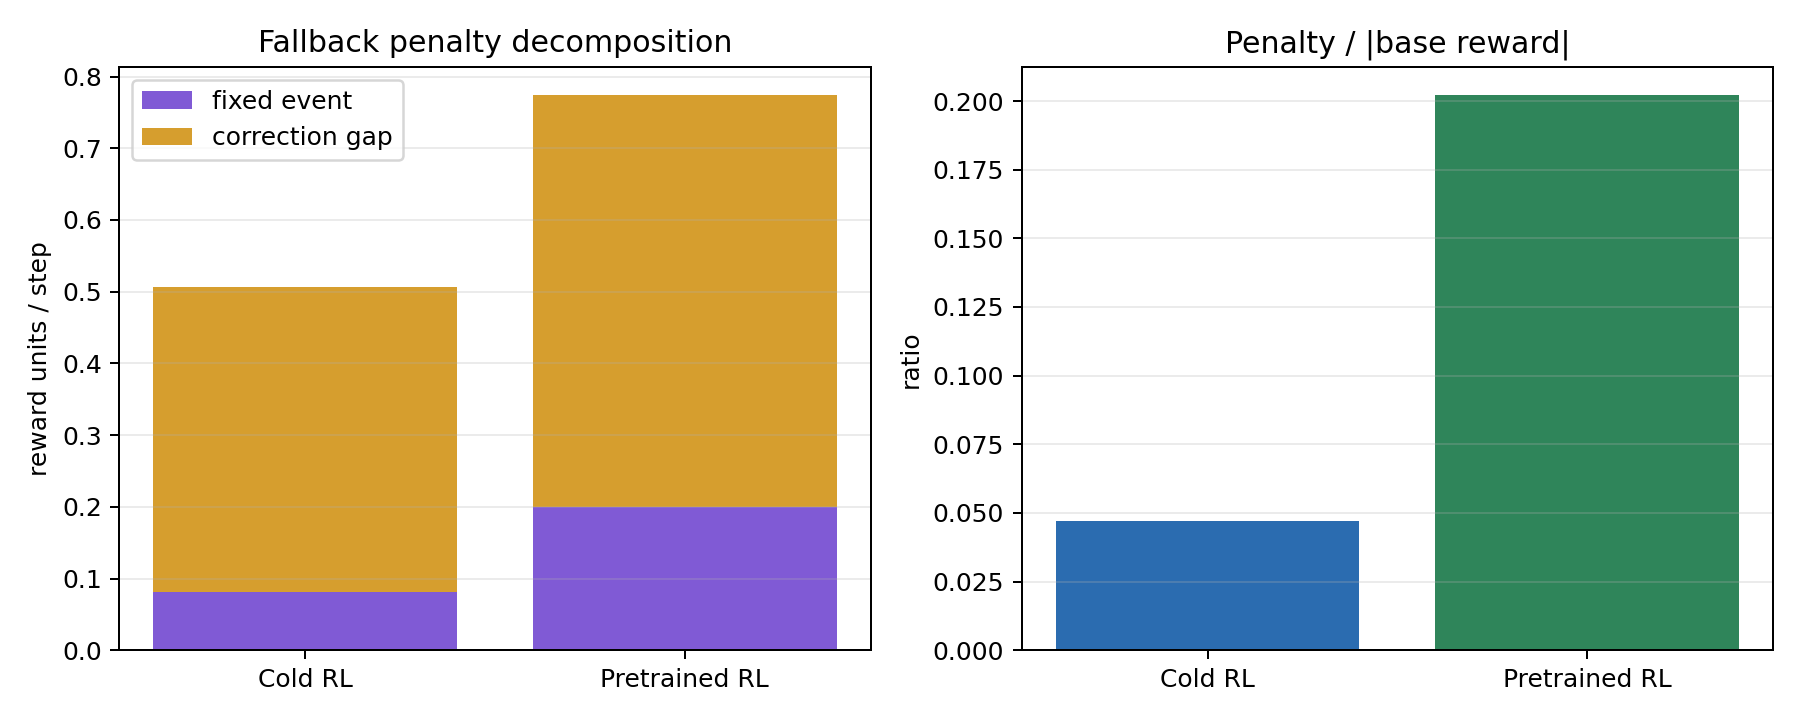
\includegraphics[width=\textwidth]{reward_penalty_scale.png}
\end{column}
\end{columns}

\takeawaybox{Fallback penalty is visible, but target quality remains the stronger limiting mechanism.}
\end{frame}

%============================= Backup 2 ============================
\begin{frame}
\frametitle{\large \textbf{Backup: activation diagnostics}}
\scriptsize

\begin{center}
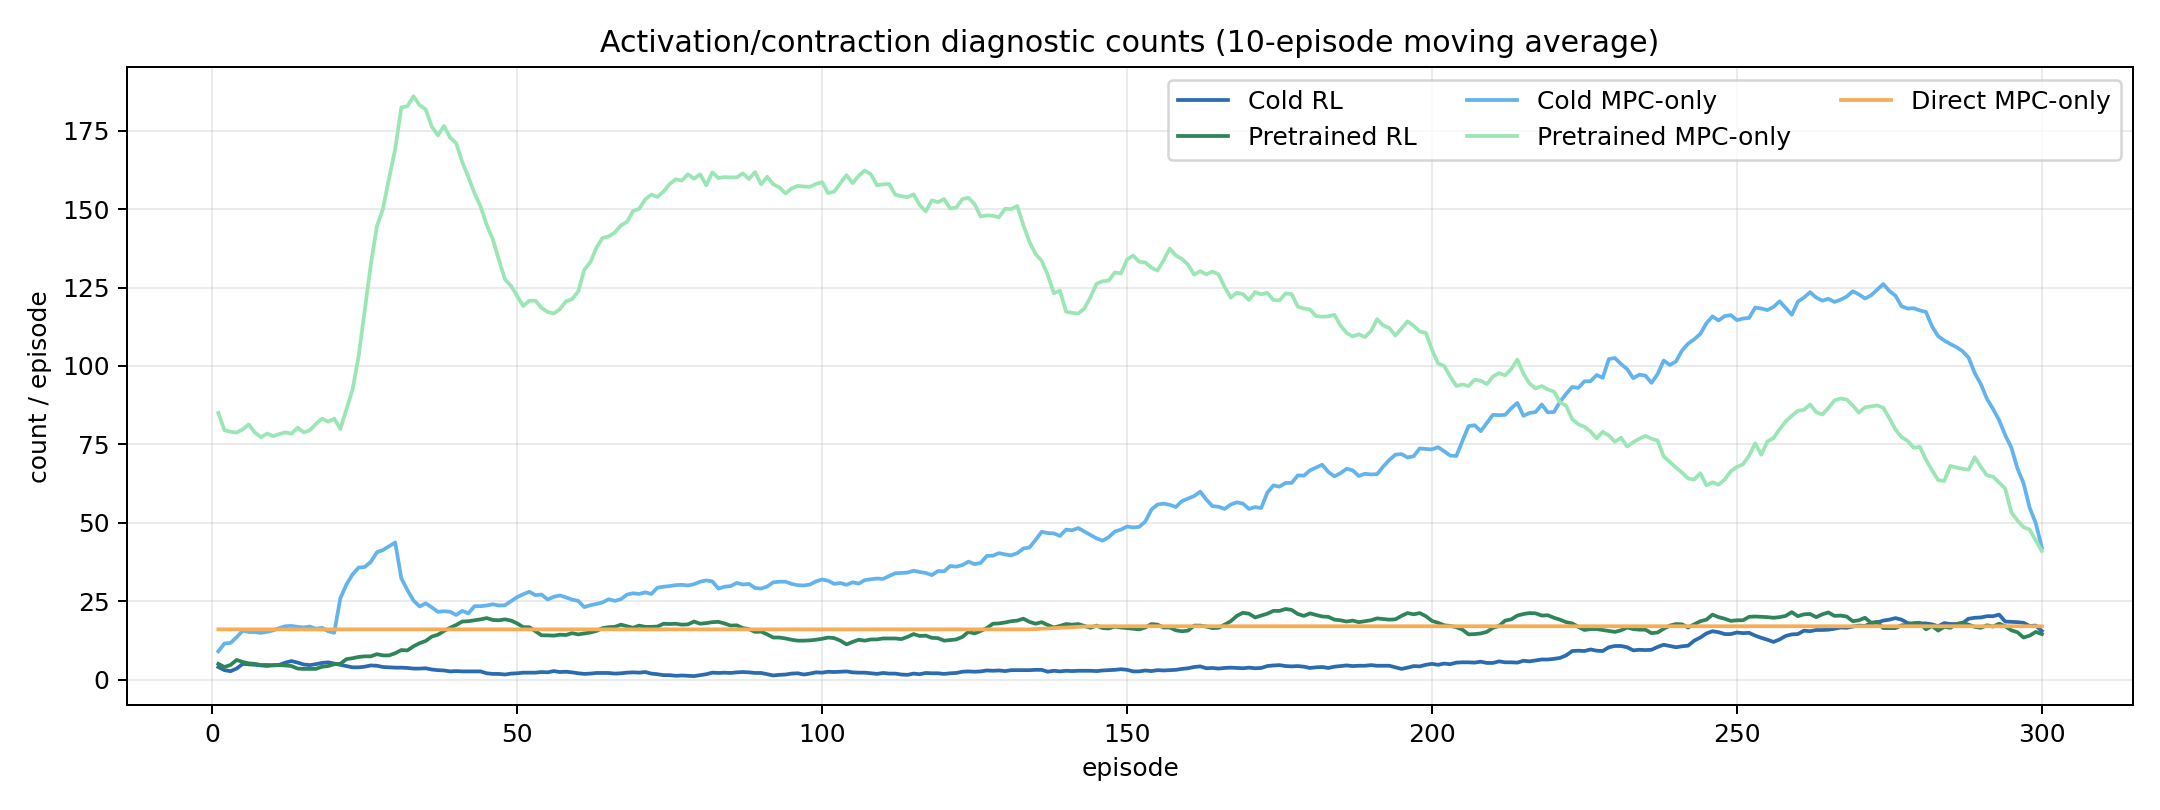
\includegraphics[width=0.86\textwidth]{activation_contraction_episode_counts.png}
\end{center}

\begin{block}{MPC-only convention}
\justifying
For MPC-only rows, actual fallback is zero by construction. The useful number is the would-be Lyapunov activation rate if the same gate were active.
\end{block}

\takeawaybox{MPC-only fallback should not be plotted as zero unless the plot explicitly means actual fallback.}
\end{frame}

%============================= Backup 3 ============================
\begin{frame}
\frametitle{\large \textbf{Backup: target diagnostics summary}}
\scriptsize

\begin{center}
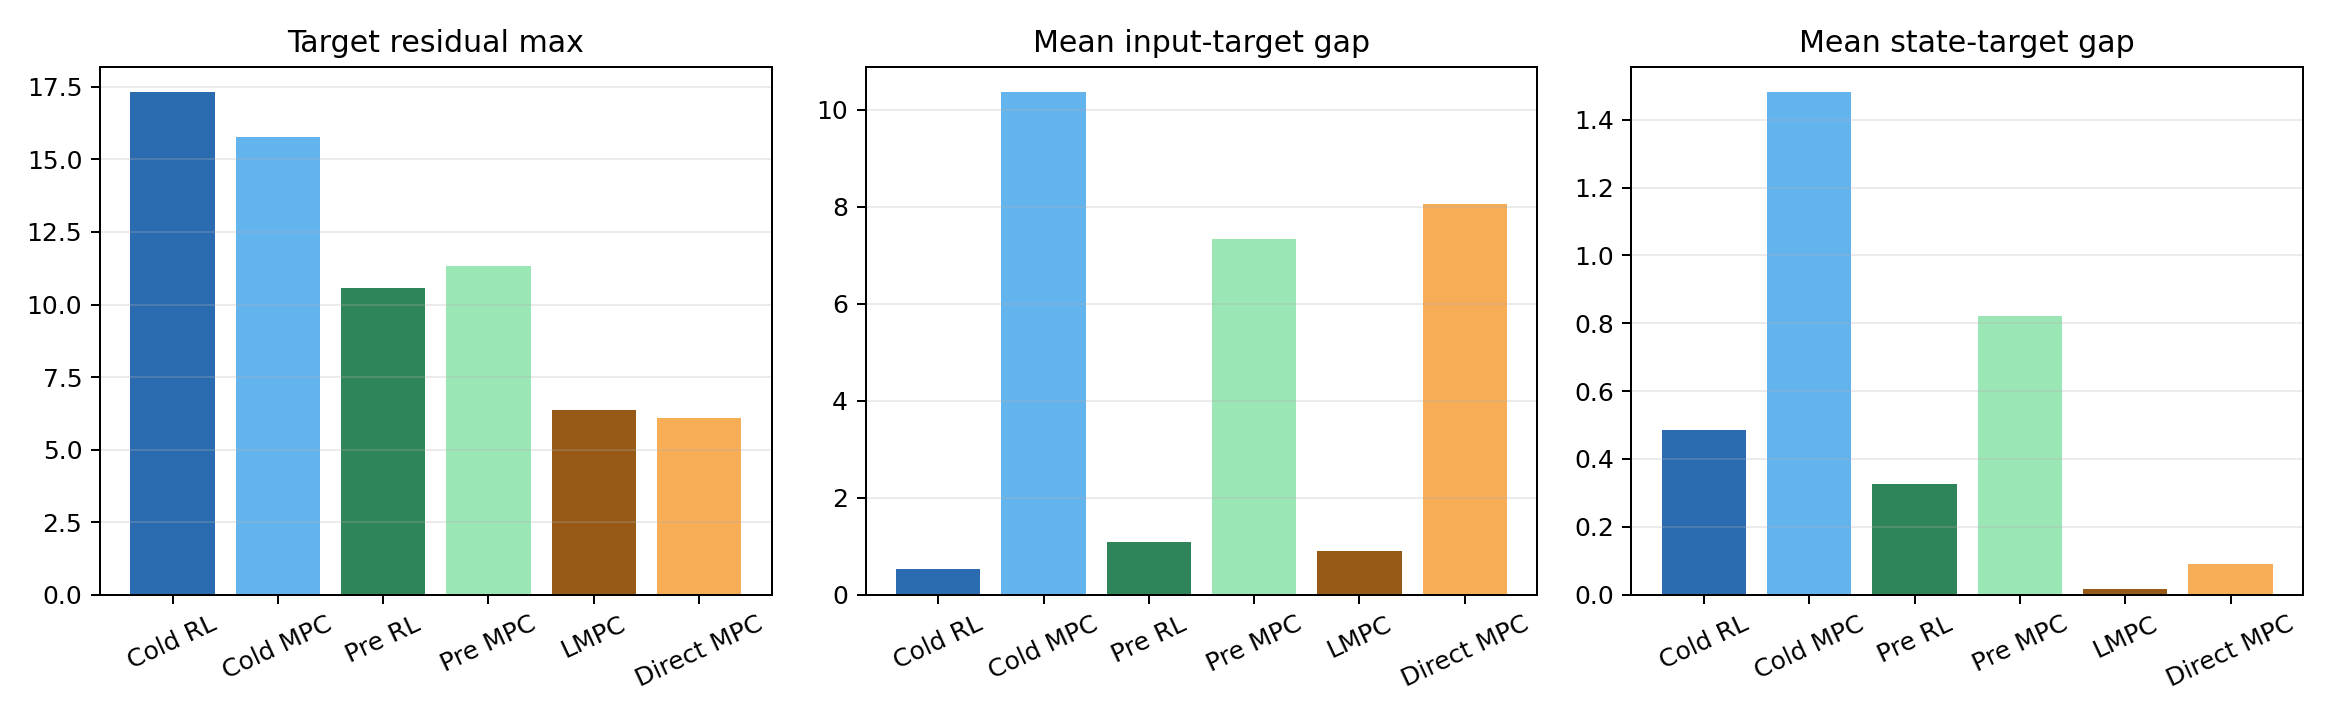
\includegraphics[width=0.88\textwidth]{target_diagnostics_summary.png}
\end{center}

\begin{block}{Interpretation}
\justifying
The direct no-RL cases can have lower target residuals while showing worse raw-setpoint RMSE. This is the key evidence that target feasibility and raw tracking alignment are not the same property.
\end{block}
\end{frame}

%============================= Backup 4 ============================
\begin{frame}
\frametitle{\large \textbf{Backup: ideas already tried or implemented}}
\scriptsize

\begin{columns}[T,onlytextwidth]
\begin{column}{0.48\textwidth}
\begin{block}{Do not present as new}
\begin{itemize}\justifying
  \setlength\itemsep{0.30ex}
  \item Four-mode selector surface.
  \item Selector warm-start and last-valid target backup.
  \item First-step contraction upstream MPC.
  \item $u_{\rm prev}$ anchoring and $x_s$ smoothing.
  \item Target-output tracking in RL direct-gate path.
\end{itemize}
\end{block}
\end{column}
\begin{column}{0.48\textwidth}
\begin{block}{Also already tried}
\begin{itemize}\justifying
  \setlength\itemsep{0.30ex}
  \item Fixed fallback event penalty up to 10.
  \item Maintenance and jitter penalties, now disabled.
  \item Pretrained exploration 0.02 to 0.01.
  \item Cold-start exploration 0.2 to 0.01.
  \item $\epsilon=10^{-3}$ and $\epsilon=10^{-2}$.
\end{itemize}
\end{block}
\end{column}
\end{columns}

\takeawaybox{The next proposal should change the target-selection logic in a measurable way.}
\end{frame}

%============================= Backup 5 ============================
\begin{frame}
\frametitle{\large \textbf{Backup: literature roles used in the talk}}
\scriptsize

\begin{block}{Minimal citation map}
\begin{itemize}\justifying
  \setlength\itemsep{0.45ex}
  \item MPC baseline and Lyapunov MPC language: Rawlings, Mayne, and Diehl, 2017.
  \item TD3 actor-critic background: Fujimoto, van Hoof, and Meger, 2018.
  \item Safe RL motivation: Garcia and Fernandez, 2015.
  \item Predictive safety filters: Wabersich and Zeilinger, 2021.
  \item Offset-free MPC-pretrained RL in process control: Hassanpour, Mhaskar, and Corbett, 2024.
\end{itemize}
\end{block}

\begin{block}{Citation policy for this first draft}
\justifying
The deck uses only local BibTeX entries found in \texttt{MACC2026/research\_summary\_2026\_draft.bib}. No new citation keys were invented.
\end{block}
\end{frame}

\end{document}
